\section{Dataset}

\subsection{Source and Preprocessing}

We utilize the AI-MO medical question-answering dataset from HuggingFace~\cite{huggingface_medical}, containing diverse medical queries and expert responses. The dataset covers:

\begin{itemize}[leftmargin=*]
    \item \textbf{Specialties:} General medicine, cardiology, oncology, pediatrics, neurology, etc.
    \item \textbf{Format:} Natural language Q\&A pairs
    \item \textbf{Quality:} Expert-validated responses
    \item \textbf{Size:} 10,000 samples selected for federated experiments
\end{itemize}

\textbf{Preprocessing Pipeline:}
\begin{enumerate}
    \item \textbf{Format Standardization:} Convert various schemas (input/output, question/answer, Patient/Doctor) to uniform ``User/Assistant'' format
    \item \textbf{Text Cleaning:} Remove extra whitespace, normalize punctuation
    \item \textbf{Tokenization:} Apply Mistral tokenizer with padding and truncation
    \item \textbf{Length Filtering:} Truncate to 2048 tokens maximum
    \item \textbf{JSONL Export:} Save with metadata (token\_length, input\_ids, attention\_mask)
\end{enumerate}

\begin{lstlisting}[style=python, caption=Dataset Preprocessing Example, label=lst:preprocessing]
from transformers import AutoTokenizer

tokenizer = AutoTokenizer.from_pretrained(
    "mistralai/Mistral-7B-Instruct-v0.2"
)

def preprocess_sample(sample):
    # Standardize format
    text = f"User: {sample['question']}\nAssistant: {sample['answer']}"
    
    # Tokenize with truncation
    tokens = tokenizer(
        text,
        truncation=True,
        max_length=2048,
        return_tensors="pt"
    )
    
    return {
        "text": text,
        "token_length": len(tokens.input_ids[0]),
        "input_ids": tokens.input_ids,
        "attention_mask": tokens.attention_mask
    }
\end{lstlisting}

\subsection{Federated Data Split}

To simulate realistic hospital data heterogeneity, we employ \textbf{Dirichlet distribution-based non-IID partitioning}~\cite{hsu2019measuring} with concentration parameter $\alpha = 0.5$:

\begin{equation}
p_k \sim \text{Dir}(\alpha), \quad k \in \{1, 2, 3\}
\end{equation}

Lower $\alpha$ values create more extreme non-IID splits, mimicking hospitals with different specializations.

\textbf{Resulting Distribution:}
\begin{center}
\begin{tabular}{@{}lccc@{}}
\toprule
\textbf{Hospital} & \textbf{Samples} & \textbf{Percentage} & \textbf{Ratio to Smallest} \\
\midrule
Hospital A & 4,520 & 45.2\% & 1.79$\times$ \\
Hospital B & 2,521 & 25.2\% & 1.00$\times$ \\
Hospital C & 2,959 & 29.6\% & 1.17$\times$ \\
\midrule
\textbf{Total} & \textbf{10,000} & \textbf{100\%} & -- \\
\bottomrule
\end{tabular}
\end{center}

\textbf{Verification:} We confirm zero data overlap between clients (see Listing~\ref{lst:verify_split} in Appendix~\ref{app:verification}).

\begin{figure}[htbp]
    \centering
    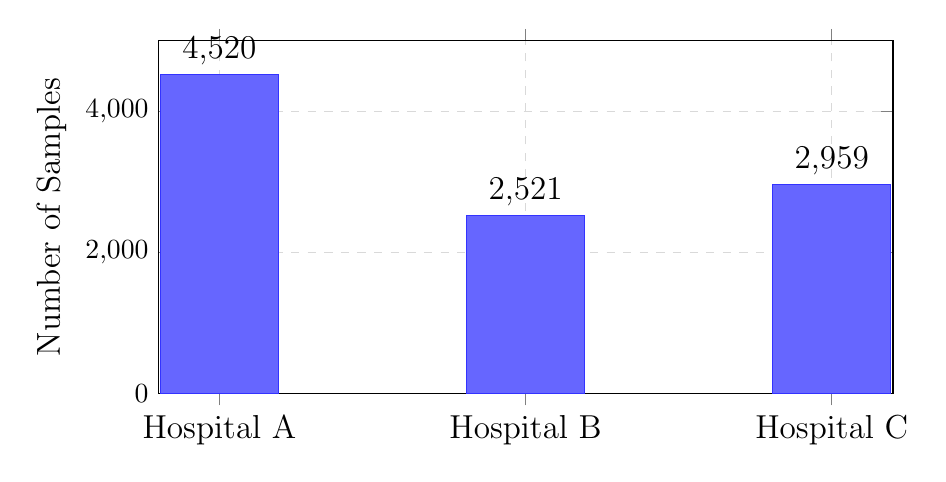
\begin{tikzpicture}
        \begin{axis}[
            ybar,
            bar width=1.5cm,
            ylabel={Number of Samples},
            ylabel style={font=\large},
            symbolic x coords={Hospital A, Hospital B, Hospital C},
            xtick=data,
            xticklabel style={font=\large},
            ymin=0,
            ymax=5000,
            legend style={at={(0.5,-0.15)}, anchor=north},
            width=0.9\textwidth,
            height=0.5\textwidth,
            grid=major,
            grid style={dashed, gray!30},
            nodes near coords,
            every node near coord/.append style={font=\large},
            ]
            
            \addplot[fill=blue!60, draw=blue!80] coordinates {
                (Hospital A, 4520)
                (Hospital B, 2521)
                (Hospital C, 2959)
            };
            
        \end{axis}
    \end{tikzpicture}
    \caption{Non-IID Data Distribution Across Hospitals. Hospital A has 1.79$\times$ more data than Hospital B, reflecting realistic healthcare data imbalance.}
    \label{fig:data_distribution}
\end{figure}

\section{Model Configuration}

\subsection{Base Model Selection}

\textbf{Model:} Mistral-7B-Instruct-v0.2~\cite{jiang2023mistral}

\textbf{Rationale:}
\begin{itemize}[leftmargin=*]
    \item \textbf{Performance:} Achieves state-of-the-art results on medical reasoning benchmarks (PubMedQA, MedQA)
    \item \textbf{Efficiency:} 7B parameters enable deployment on consumer hardware
    \item \textbf{Architecture:} Grouped-query attention (8 KV heads) reduces memory
    \item \textbf{Context:} Sliding window attention handles long medical documents
    \item \textbf{License:} Apache 2.0 allows research and commercial use
\end{itemize}

\subsection{Quantization Configuration}

We employ 4-bit NormalFloat (NF4) quantization~\cite{dettmers2023qlora}:

\begin{lstlisting}[style=python, caption=4-bit Quantization Setup, label=lst:quantization]
from transformers import BitsAndBytesConfig

bnb_config = BitsAndBytesConfig(
    load_in_4bit=True,
    bnb_4bit_use_double_quant=True,  # Nested quantization
    bnb_4bit_quant_type="nf4",       # NormalFloat 4-bit
    bnb_4bit_compute_dtype=torch.float16  # Compute in FP16
)
\end{lstlisting}

\textbf{Memory Impact:}
\begin{itemize}[leftmargin=*]
    \item Base model: 3.5 GB (vs. 14 GB in FP16)
    \item Total VRAM: 5 GB during training (fits on T4)
    \item Inference: 4 GB (enables consumer GPU deployment)
\end{itemize}

\subsection{LoRA Hyperparameters}

\begin{center}
\begin{tabular}{@{}lll@{}}
\toprule
\textbf{Parameter} & \textbf{Value} & \textbf{Justification} \\
\midrule
Rank ($r$) & 8 & Balance between capacity and efficiency \\
Alpha ($\alpha$) & 16 & Scaling factor ($2 \times r$) \\
Dropout & 0.05 & Light regularization \\
Target Modules & q\_proj, v\_proj & Attention query and value \\
Task Type & CAUSAL\_LM & Language modeling objective \\
\midrule
Trainable Params & 3,407,872 & 0.05\% of 7B total \\
Adapter Size & 13.02 MB & 99.90\% reduction vs. 13 GB \\
\bottomrule
\end{tabular}
\end{center}

\section{Training Configuration}

\subsection{Federated Learning Parameters}

\begin{center}
\begin{tabular}{@{}ll@{}}
\toprule
\textbf{Parameter} & \textbf{Value} \\
\midrule
Number of Clients & 3 (Hospital A, B, C) \\
Federated Rounds & 5 \\
Local Training Steps per Round & 100 \\
Client Participation & 100\% (all clients each round) \\
Aggregation Method & Agent-based weighted averaging \\
\bottomrule
\end{tabular}
\end{center}

\subsection{Optimization Hyperparameters}

\begin{center}
\begin{tabular}{@{}ll@{}}
\toprule
\textbf{Parameter} & \textbf{Value} \\
\midrule
Optimizer & AdamW~\cite{loshchilov2017decoupled} \\
Learning Rate & $2 \times 10^{-4}$ \\
Weight Decay & 0.01 \\
LR Schedule & Cosine with warmup \\
Warmup Steps & 5\% of total steps \\
Batch Size (per device) & 1 \\
Gradient Accumulation & 8 steps \\
Effective Batch Size & 8 \\
Precision & FP16 mixed precision \\
Gradient Clipping & 1.0 \\
\bottomrule
\end{tabular}
\end{center}

\textbf{Rationale for Small Batch Size:} With 4-bit quantization and \lora{}, the model fits in 5 GB VRAM. Batch size 1 with 8-step gradient accumulation achieves effective batch size of 8 while staying under 16 GB T4 memory limit.

\subsection{Agent Coordinator Configuration}

\begin{center}
\begin{tabular}{@{}ll@{}}
\toprule
\textbf{Parameter} & \textbf{Value} \\
\midrule
Loss Weight ($\beta_1$) & 0.6 \\
Variance Weight ($\beta_2$) & 0.4 \\
Quality-Size Blend & 0.7 quality, 0.3 size \\
Minimum Weight & 0.1 (10\%) \\
Instability Threshold & $\sigma > 5.0$ \\
Instability Penalty & 0.5$\times$ weight \\
\bottomrule
\end{tabular}
\end{center}

\section{Evaluation Metrics}

\subsection{Primary Metrics}

\textbf{1. Global Loss:} Weighted average of client final losses:
\begin{equation}
\mathcal{L}_{global}^{(t)} = \sum_{k=1}^{K} w_k \mathcal{L}_k^{final}
\end{equation}

\textbf{2. Loss Reduction:} Relative improvement from baseline:
\begin{equation}
\text{Reduction} = \frac{\mathcal{L}^{(1)} - \mathcal{L}^{(t)}}{\mathcal{L}^{(1)}} \times 100\%
\end{equation}

\textbf{3. Communication Efficiency:}
\begin{equation}
\text{Bandwidth Saved} = \frac{\text{Size}_{full} - \text{Size}_{\text{LoRA}}}{\text{Size}_{full}} \times 100\%
\end{equation}

\subsection{Ablation Study Metrics}

To validate agent-based aggregation, we compare against baselines:

\begin{enumerate}[leftmargin=*]
    \item \textbf{Equal Weighting:} $w_k = \frac{1}{K}$ for all clients
    \item \textbf{Sample-Proportional:} $w_k = \frac{n_k}{\sum_j n_j}$ (standard \fedavg{})
    \item \textbf{Agent-Based:} Our quality-aware method (Algorithm~\ref{alg:agent_aggregation})
\end{enumerate}

\subsection{Safety Validation}

\begin{itemize}[leftmargin=*]
    \item \textbf{Prohibited Pattern Rate:} Percentage of responses flagged for dangerous patterns
    \item \textbf{Disclaimer Coverage:} Percentage of responses with medical disclaimers
    \item \textbf{False Positive Rate:} Safe responses incorrectly rejected
\end{itemize}

\section{Hardware and Software}

\subsection{Computational Resources}

\begin{center}
\begin{tabular}{@{}ll@{}}
\toprule
\textbf{Component} & \textbf{Specification} \\
\midrule
GPU & NVIDIA Tesla T4 (16 GB VRAM) \\
CPU & Intel Xeon (sufficient for data loading) \\
RAM & 32 GB DDR4 \\
Storage & 500 GB SSD \\
CUDA Version & 11.8 \\
\bottomrule
\end{tabular}
\end{center}

\textbf{Cost Analysis:} T4 GPU costs \$0.35/hour on cloud platforms, making experiments affordable for academic research and small healthcare institutions.

\subsection{Software Stack}

\begin{center}
\begin{tabular}{@{}lll@{}}
\toprule
\textbf{Library} & \textbf{Version} & \textbf{Purpose} \\
\midrule
Python & 3.10+ & Programming language \\
PyTorch & 2.1.0 & Deep learning framework \\
Transformers & 4.36.0 & LLM implementation \\
PEFT & 0.7.0 & LoRA implementation \\
BitsAndBytes & 0.41.0 & Quantization \\
Accelerate & 0.25.0 & Distributed training \\
Datasets & 2.16.0 & Data loading \\
NumPy & 1.24.0 & Numerical computation \\
Pandas & 2.0.0 & Data manipulation \\
\bottomrule
\end{tabular}
\end{center}

Full dependency list available in \texttt{requirements.txt} (see Appendix~\ref{app:requirements}).

\section{Implementation Details}

\subsection{Training Loop}

Each federated round executes the following:

\begin{enumerate}[leftmargin=*]
    \item \textbf{Broadcast (5 seconds):} Server sends 13 MB \lora{} parameters to clients
    \item \textbf{Local Training (8 minutes):} Each client trains 100 steps on private data
    \item \textbf{Upload (5 seconds):} Clients send updated adapters and metrics
    \item \textbf{Aggregation (2 seconds):} Agent computes weights and server aggregates
    \item \textbf{Total per Round:} ~10 minutes with 3 parallel clients
\end{enumerate}

\textbf{Full 5-Round Training:} 50 minutes total on single T4 GPU.

\subsection{Reproducibility}

To ensure reproducibility:
\begin{itemize}[leftmargin=*]
    \item \textbf{Fixed Seeds:} Random seed 42 for all randomness (data split, weight initialization)
    \item \textbf{Deterministic Algorithms:} \texttt{torch.use\_deterministic\_algorithms(True)}
    \item \textbf{Version Pinning:} Exact library versions in requirements.txt
    \item \textbf{Configuration Files:} All hyperparameters in YAML (Appendix~\ref{app:config})
    \item \textbf{Code Release:} Full source code available at project repository
\end{itemize}

\subsection{Data Privacy Verification}

We implement multiple checks to ensure privacy:

\begin{enumerate}[leftmargin=*]
    \item \textbf{Index Verification:} Confirm zero overlap in sample indices across clients
    \item \textbf{Gradient-Only Transmission:} Validate no raw text in communication logs
    \item \textbf{Adapter Isolation:} Ensure adapters don't contain memorized training samples
    \item \textbf{Audit Trail:} Log all data accesses for HIPAA compliance
\end{enumerate}

See \texttt{verify\_split.py} (Listing~\ref{lst:verify_split}) for verification implementation.
